As defined in Section~\ref{sec:intro}, let (i) the Hybrid Pedal Curve $\mathcal{E}^*$ be the locus of the intersection $Q^*$ of $\mathcal{L}(t)$ with the line from $M$ to $Q_p$, Figure~\ref{fig:hybrid}, and (ii) the Pseudo Talbot Curve $\mathcal{E}^\dagger$ be  the Negative Pedal Curve of $\mathcal{E}^*$, Figure~\ref{fig:hybrid-npc}. Here we prove their area invariance over all $M$ on $\mathcal{E}$.

\begin{theorem}
	The area $A^*$ of $\mathcal{E}^*$ is invariant for all $M$ on $\mathcal{E}$ and given by:
	\[ A^*= \frac{\pi  (3a^4+2a^2b^2+3b^4)}{2 a b}=\frac{\pi(3\delta^2+5a^2b^2)}{2 a b},\;\; \delta=\sqrt{a^4-a^2b^2+b^4}
	\]
%\label{thm:area-hybrid}
\end{theorem}

\begin{proof}

Let $P(t)=[a\cos{t},b\sin{t}]$ be a point on $\mathcal{E}$. By definition (Section~\ref{sec:intro} and  Figure~\ref{fig:hybrid}), $\mathcal{E}^*$ is defined as the intersection of lines
\[ M+ uP'(t)^{\perp}\;\;\; \text{and}\;\;\; P(t)+v (M-P(t))^{\perp}.\]

\noindent Let $M=[x_0,y_0]$ and $\mathcal{E}(t)=[x^*(t),y^*(t)]$. Straightforward calculation leads to:

{\small
\begin{align*}
x^*(t)=&\frac{
-b\left(3{a}^{2}+{b}^{2}+4{y_0}^{2}\right)\cos{t}
+4{a}{b}{x_0}\cos{2{t}}
-b c^2 \cos{3{t}}
+4{a}{x_0}{y_0}\sin{t}
+4{b}^{2}{y_0}\sin{2{t}}
}{
4\left(a{y_0}\sin{t}+b{x_0}\cos{t}-{a}{b}\right)
}\\
y^*(t)=&\frac{
-a\left({a}^{2}+3{b}^{2}+4{x_0^{2}}\right)\sin{t}
+4{a}^{2}{x_0}\sin{2{t}}
-a c^2\sin{3{t}}
+4{b}{x_0}{y_0}\cos{t}
-4{a}{b}{y_0}\cos{2{t}}
}{
4\left(a{y_0}\sin{t}+b{x_0}\cos{t}-{a}{b}\right)
}
\end{align*}
}

\noindent where $c^2=a^2-b^2$. Integrating Equation~\ref{eqn:area} over $\mathcal{E}^*(t)$ yields the claim.
\end{proof}

\begin{figure}
    \centering
    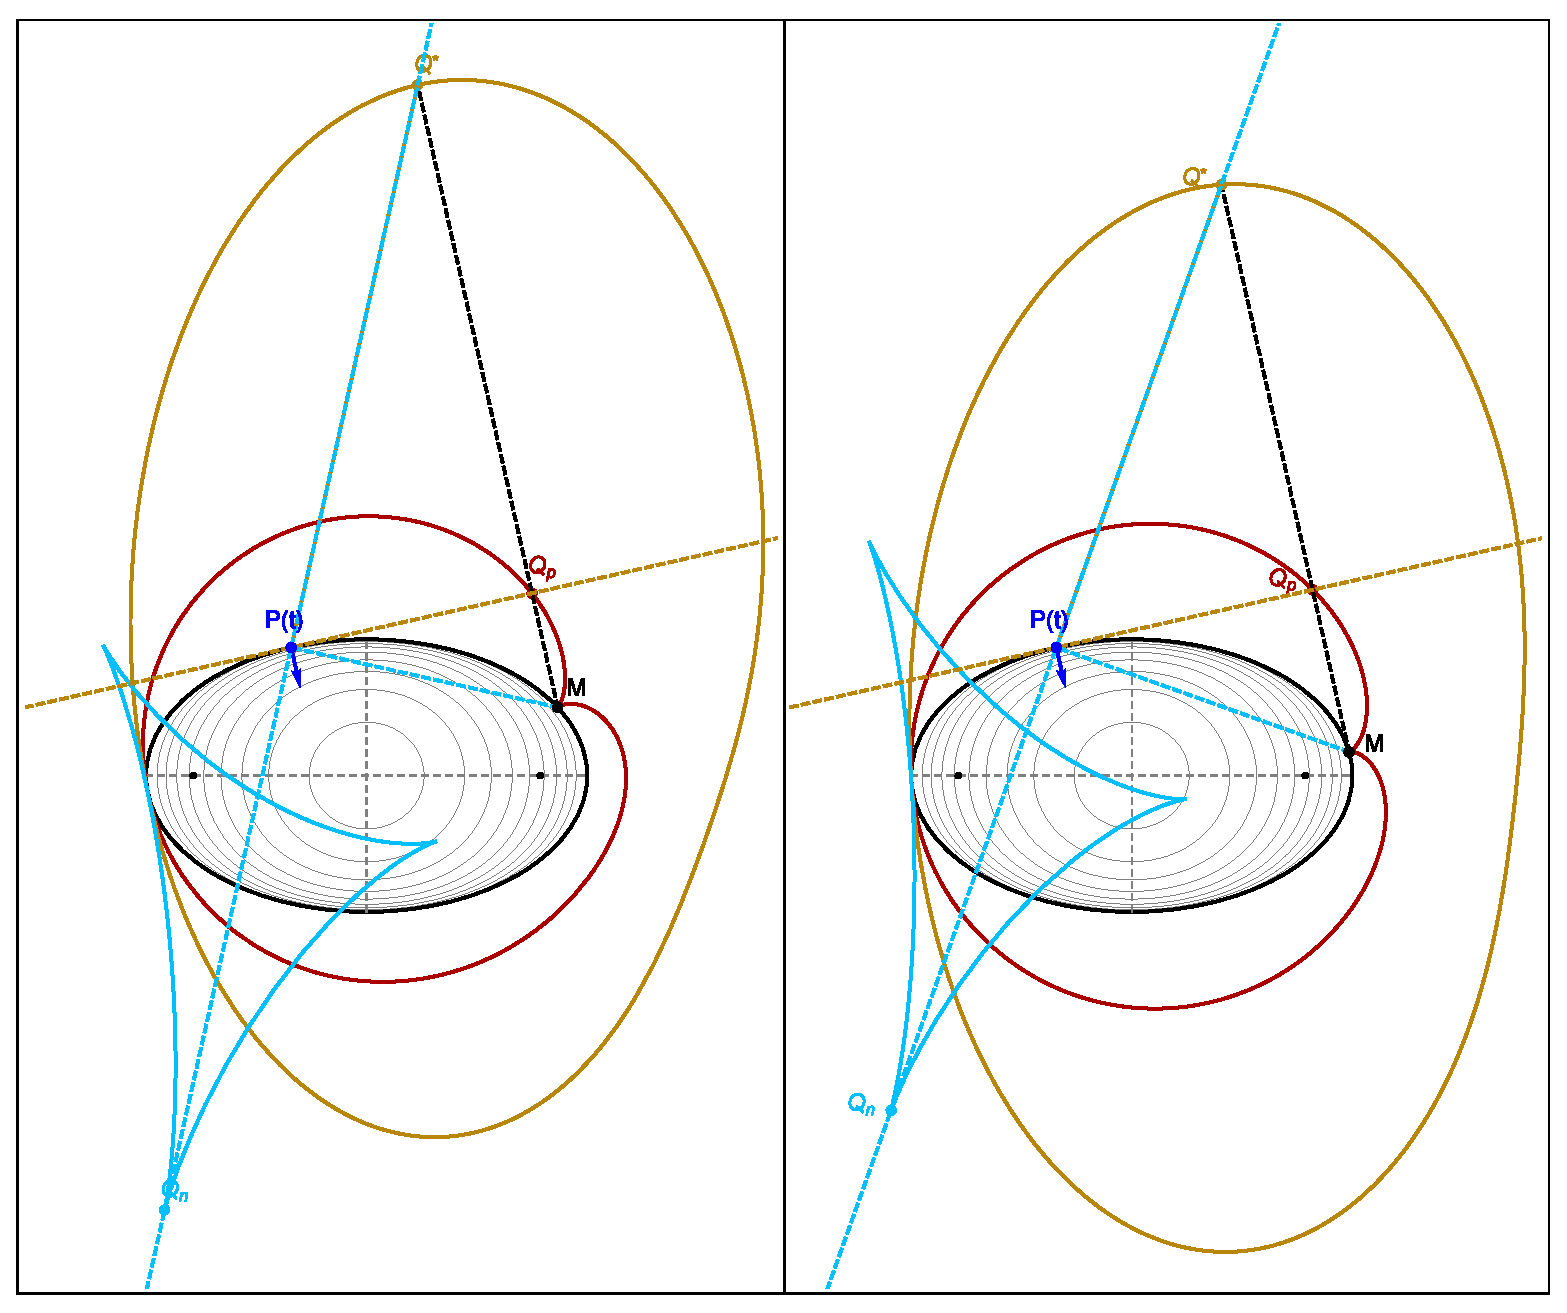
\includegraphics[width=\textwidth]{pics/0040_hybrid_curve.eps}
    \caption{The Pedal $\mathcal{E}_p$ (red) and Hybrid Pedal $\mathcal{E}^*$ (light brown), and Negative-Pedal $\mathcal{E}_n$ (light blue) Curves of the ellipse $\mathcal{E}$ (black) shown for two positions of $M$. $\mathcal{E}^*$ is the locus of the intersection $Q^*$ of (i) the line through $P(t)$ perpendicular to $P(t)-M$ and (ii) line $M{Q_p}$ (note $\mathcal{E}_p$ is the locus of $Q_p$). For both left and right pictures (indeed for all $M$ on the ellipse), areas $A_n,A^*$ are constant, although that of $\mathcal{E}_p$ varies. Also shown are iso-curves of constant $A^*$ inside the ellipse; these are high-order rational curves. $\mathcal{E}^*$ is unstable when $M$ is exterior to $\mathcal{E}$.}
    \label{fig:hybrid}
\end{figure}

\begin{theorem}
The area $A^\dagger$ of $\mathcal{E}^\dagger$ is invariant for all $M$ on $\mathcal{E}$ and given by:
	
	\[ A^\dagger=  -  \frac {\pi\, \left( 3\,{a}^{4}+2\,{a}^{2}{b}^{2}+3\,{b}^{4}
 \right)  \left( {a}^{2}-2\,ab-{b}^{2} \right)  \left( {a}^{2}+2\,ab-{
b}^{2} \right) }{8 a^{3} b^{3}}
	\]
%\label{thm:area-talbot}
\end{theorem}

\begin{proof}
Recall $\mathcal{E}^\dagger$ is the negative pedal curve of $\mathcal{E}^*$ (Section~\ref{sec:intro} and Figure~\ref{fig:hybrid-npc}). For $M=[a\cos u,b\sin u]$ on the ellipse, the coordinates $[x^\dagger,y^\dagger]$ of $\mathcal{E}^\dagger$ can be derived explicitly:

{\small  
\begin{align*}
x^{\dagger}(u)=&\frac{\left(c^4(2\cos(2t) - \cos(4t)) - (a^2 - 3b^2)(a^2 + b^2)\right)\cos{u} }{4 a b^2} - \frac{2c^4 \sin^3t \cos{t} \sin{u}}{a b^2}\\
&+ \frac{(a^2 + b^2)(b^2-c^2\sin^2{t}  )\cos{t}}{a b^2}\\
y^{\dagger}(u)=&-\frac{2c^4 \sin{t} \cos^3{t}\cos{u}}{a^2b} - \frac{(c^4(2\cos(2t) + \cos(4t)) - (3a^2 - b^2)(a^2 + b^2))\sin{u}}{ 4a^2b}\\
&+\frac{  (a^2 + b^2)(c^2 \cos^2{t}    + a^2)\sin{t}}{a^2 b}
\end{align*}
}

Integrating Equation~\eqref{eqn:area} for the above yields the claimed results.
\end{proof}

\begin{figure}
    \centering
    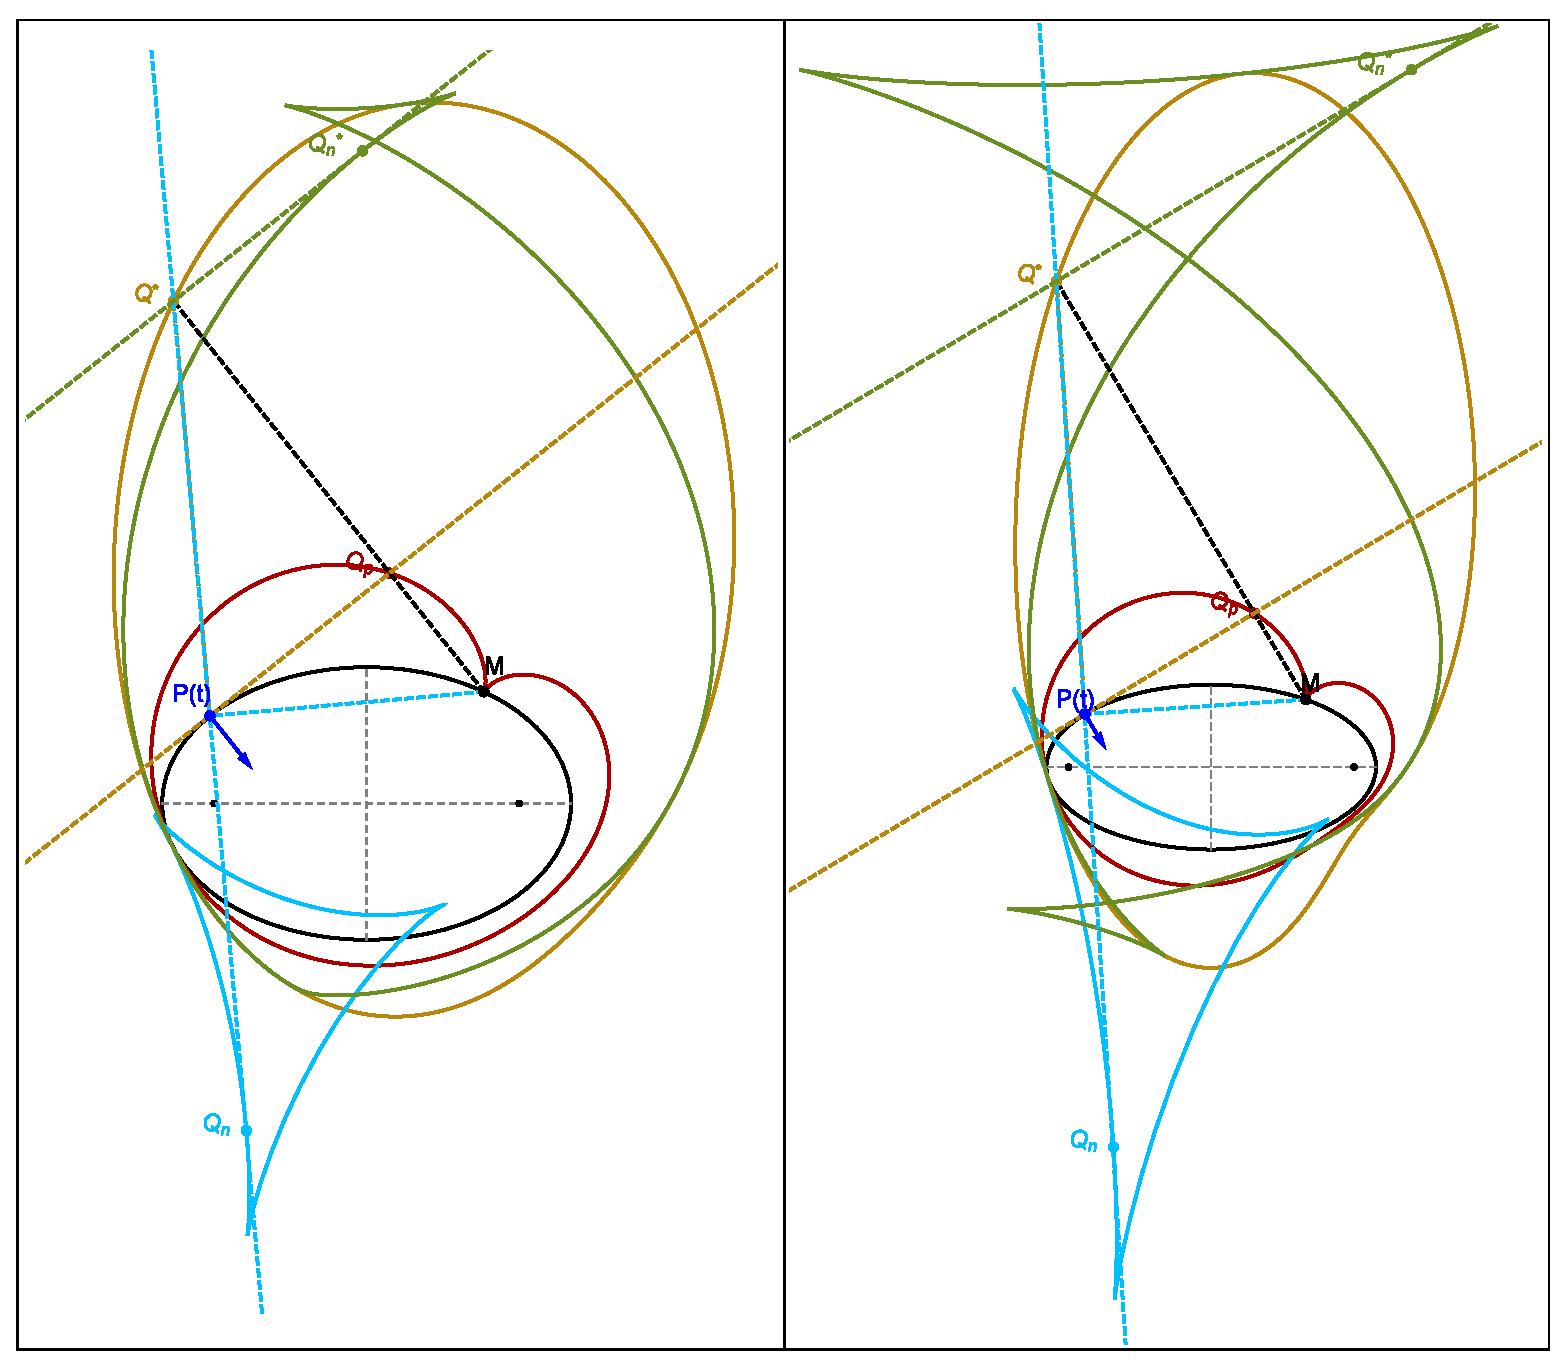
\includegraphics[width=\textwidth]{pics/0060_hybrid_npc.eps}
    \caption{The pedal, negative pedal, hybrid pedal $\mathcal{E}^*$, and pseudo-Talbot curve $\mathcal{E}^\dagger$ (negative pedal curve of $\mathcal{E}^*$) are shown red, light blue, brown, and olive green, respectively, for aspect ratios $a/b$ of $\mathcal{E}$ of 1.5 (left) and 2.0 (right), respectively. Notice that for the former case $\mathcal{E}^\dagger$ has two cusps, and in the latter 4. Excluding the pedal curve, all other 3 are area-invariant for $M$ on $\mathcal{E}$, and are all tangent to $\mathcal{E}$ at the point where the normal goes through $M$.}
    \label{fig:hybrid-npc}
\end{figure}


